\documentclass[border=4pt]{standalone}

% --- packages (mirror these in cpu.meta.json "requires") ---
\usepackage{tikz}

% --- palette (canonical source: reference/color-palettes/color-palettes.md; light variant) ---
\definecolor{otblue}{HTML}{0072B2}
\definecolor{otorange}{HTML}{E69F00}
\definecolor{otteal}{HTML}{009E73}
\definecolor{otpurple}{HTML}{CC79A7}
\definecolor{otgray}{HTML}{5A5A5A}

\begin{document}
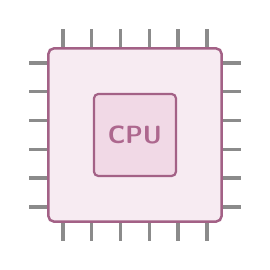
\begin{tikzpicture}
  \def\s{1.1}        % half side of the chip body
  \def\pinlen{0.24}  % pin length
  \def\np{6}         % pins per side
  % pins (behind the body)
  \foreach \i in {1,...,\np}{
    \pgfmathsetmacro{\p}{-\s + 2*\s*(\i-0.5)/\np}
    \draw[otgray!70, line width=1.3pt] (\p,\s)  -- (\p,\s+\pinlen);
    \draw[otgray!70, line width=1.3pt] (\p,-\s) -- (\p,-\s-\pinlen);
    \draw[otgray!70, line width=1.3pt] (\s,\p)  -- (\s+\pinlen,\p);
    \draw[otgray!70, line width=1.3pt] (-\s,\p) -- (-\s-\pinlen,\p);
  }
  % chip body
  \filldraw[draw=otpurple!80!black, fill=otpurple!15, rounded corners=2pt, line width=0.9pt]
    (-\s,-\s) rectangle (\s,\s);
  % core
  \filldraw[draw=otpurple!80!black, fill=otpurple!28, rounded corners=1.5pt, line width=0.8pt]
    (-0.52,-0.52) rectangle (0.52,0.52);
  \node[font=\sffamily\small\bfseries, text=otpurple!85!black] at (0,0) {CPU};
\end{tikzpicture}
\end{document}
